\Subhead{1.11.1}{Хаотические колебания. Понятие о хаотическом (странном) аттракторе}
\textbf{Определение и физический смысл.} Детерминированный хаос --- ограниченное нерегулярное движение, возникающее по однозначным динамическим законам и обладающее чувствительностью к начальным условиям. Знание уравнения не позволяет предсказывать отдельную траекторию бесконечно долго при конечной точности исходных данных. При этом статистические характеристики могут оставаться воспроизводимыми. Хаос отличается от заданного извне случайного шума, хотя экспериментальный сигнал обычно содержит оба вклада.

\paragraph{Аттрактор и показатели Ляпунова.}
Аттрактор --- инвариантное множество, притягивающее некоторую область начальных условий. Странный аттрактор характеризуется сложной, часто фрактальной геометрией; для хаотического режима существенна также динамическая неустойчивость траекторий на нём. Геометрическое слово «странный» само по себе не заменяет проверку хаоса: существуют и странные нехаотические аттракторы.

Линеаризованное возмущение удовлетворяет $\delta\dot{\bm z}=J(\bm z(t))\delta\bm z$. Максимальный показатель
\begin{equation}
 \lambda_{\max}=\lim_{t\to\infty}\frac1t\ln
 \frac{\|\delta\bm z(t)\|}{\|\delta\bm z(0)\|}
\end{equation}
определяется вдоль траектории с периодической перенормировкой малого вектора, чтобы сохранять линейность вариационного уравнения. Положительное значение в ограниченном установившемся режиме свидетельствует об экспоненциальном разделении близких траекторий до масштаба аттрактора. Горизонт прогноза примерно $t_{\mathrm{pred}}\sim\lambda_{\max}^{-1}\ln(\Delta_{\mathrm{allow}}/\Delta_0)$. Рост расстояния не продолжается неограниченно: аттрактор ограничен, а растяжение сочетается со складыванием траекторий.

Для гладкого автономного потока на плоскости при обычных условиях теоремы Пуанкаре--Бендиксона хаотический аттрактор невозможен. Нужна как минимум третья переменная либо иной механизм: внешняя периодическая сила, запаздывание или дискретное отображение. Периодически возбуждаемый осциллятор второго порядка становится трёхмерной автономной системой после добавления фазы силы. Одномерное \emph{отображение} не подчиняется этому ограничению для непрерывного потока.\paragraph{Пример курса и три переменные.}
В конспекте Пятакова (PDF-с.~69) приведён LC-контур с нелинейным диодом и обратной связью. Переменные состояния можно выбрать как заряд основного конденсатора $q$, ток индуктивности $I_L=\dot q$ и напряжение диодного узла $V_d$:
\begin{equation}\label{eq:diodechaos}
 \dot q=I_L,\quad
 L\dot I_L=\mathcal E_{\rm fb}(q,I_L)-RI_L-q/C-V_d,\quad
 C_1\dot V_d=I_L-I_d(V_d).
\end{equation}
Последнее равенство --- закон Кирхгофа для тока, делящегося между нелинейным диодом и его дополнительной ёмкостью $C_1$. В конспекте обратная связь задаётся через взаимную индукцию и крутизну активного элемента; здесь она обозначена $\mathcal E_{\rm fb}$. Три накопителя $L,C,C_1$ дают три переменные: одной плоской фазовой картинки недостаточно.
% Источник: Пятаков, PDF-с.69, первые уравнения контура и qdot=I+C1 Vdot.
% Обозначение E_fb введено здесь, чтобы не приписать непроверенную схему активного элемента.
 Нелинейный активный элемент поддерживает движение, а диссипация ограничивает доступный объём фазового пространства. Это физическая мотивация трёхмерной модели, а не утверждение хаоса при любых номиналах схемы.

Стандартный пример трёхмерного потока — система Лоренца
\begin{equation}
 \dot x=\sigma(y-x),\qquad \dot y=rx-y-xz,\qquad \dot z=xy-bz.
\end{equation}
При $\sigma=10$, $b=8/3$, $r=28$ численное решение после переходного процесса даёт характерный двухлепестковый аттрактор. Соседние траектории расходятся, хотя все остаются ограниченными. В лазерной аналогии переменные связаны с полем, поляризацией и инверсией; поле нельзя называть интенсивностью без изменения уравнений.

\begin{center}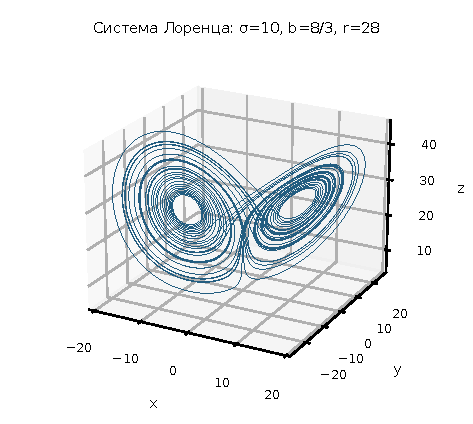
\includegraphics[width=0.76\linewidth]{figures/lorenz.pdf}\end{center}
